\begin{figure}
    \centering
    \setlength{\resLen}{0.8in}
    \addtolength{\tabcolsep}{-3pt}
    \begin{tabular}{cccc}
        \multicolumn{4}{c}{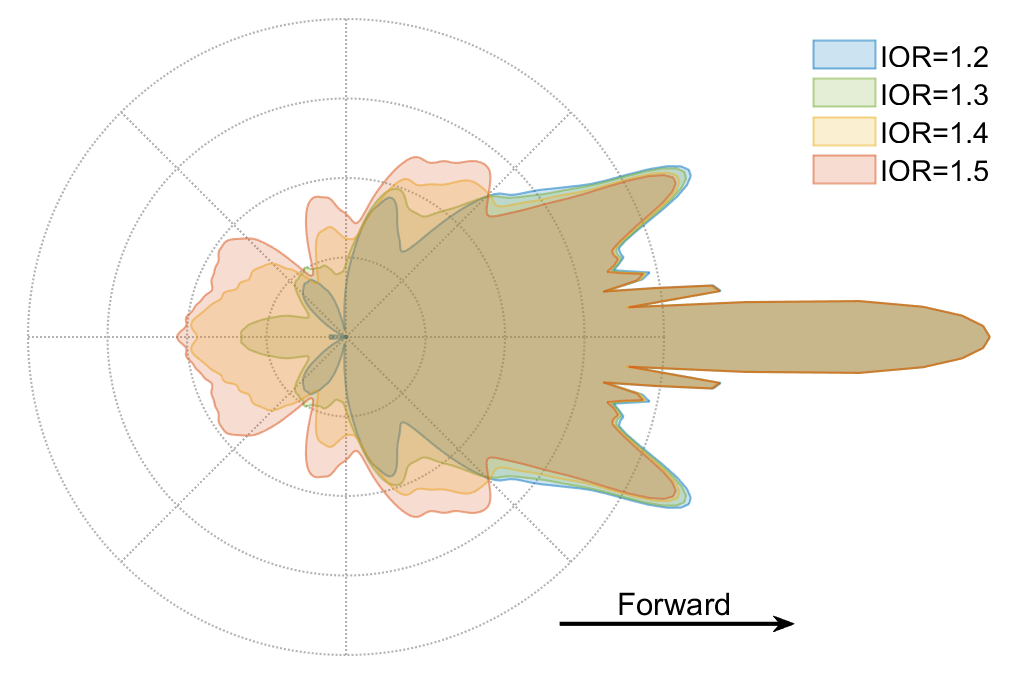
\includegraphics[height=1.8\resLen]{images/pfunc/IOR.png}} \\ [0em]
        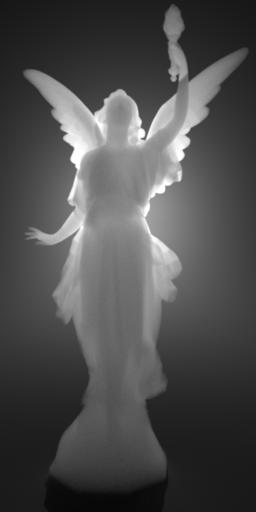
\includegraphics[width=\resLen]{images/lucy/ior_1.2.jpg} &
        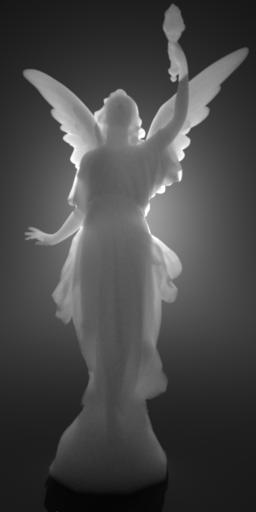
\includegraphics[width=\resLen]{images/lucy/ior_1.3.jpg} &
        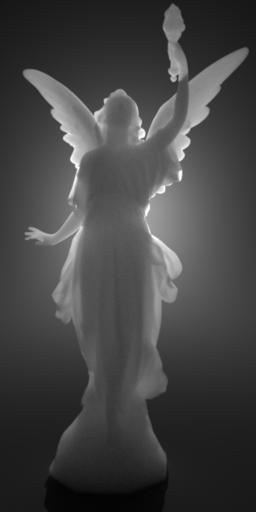
\includegraphics[width=\resLen]{images/lucy/ior_1.4.jpg} &
        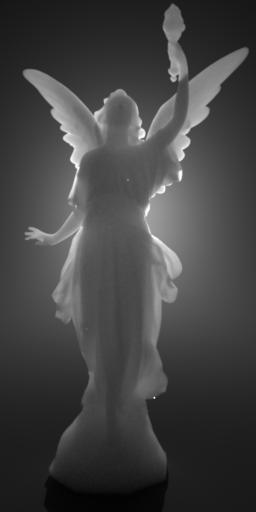
\includegraphics[width=\resLen]{images/lucy/ior_1.5.jpg} \\
        $\sIOR=1.2+0\img$ & $\sIOR=1.3+0\img$ & $\sIOR=1.4+0\img$ & $\sIOR=1.5+0\img$
    \end{tabular}
    \caption{\label{fig:ior}
        \rev{
            Effect of the refractive index of the particles. The top of this figure visualizes the bulk phase functions of clusters of 100 particles with radii 500nm. 
            The refractive index of the particles range from $\sIOR = 1.2+0\img$ to $1.5+0\img$ suspended in the vacuum. 
            The bottom figures show renderings of the Lucy model for media with each refractive index.
        }
    }
\end{figure}

